\section{Data}\label{sec:data}

This chapter provides a detailed overview of the comprehensive data collection, integration, and preprocessing efforts that underpin the empirical analyses conducted in this thesis. Accurate and reliable data is paramount in robust economic modeling, especially for evaluating policy effects with causal machine learning frameworks. Accordingly, the data incorporated in this study is exclusively drawn from high-quality, publicly available U.S. economic sources, given their superior completeness, transparency, and temporal coverage \citep{bareinboim2023, bankofcanada2023}.

\subsection{Rationale for Data Selection}

The choice to focus on United States economic data was motivated by the rich availability and documentation of official macroeconomic and microeconomic statistics. Despite exploring numerous global datasets and national statistical agencies, no alternative source provided consistent multi-year, multi-sector information integrating macro indicators with firm-level and demographic microdata at the requisite granularity \citep{garcia2020, imf2023}. Using U.S. data ensures methodological rigor, facilitates replicability, and supports nuanced heterogeneous effect analysis not commonly feasible in other regions.

\subsection{Data Sources and Collection}\label{subsec:data_sources}

The empirical dataset synthesizes several reputable sources accessed via both automated API interfaces and curated static files:

\begin{itemize}
  \item \textbf{Federal Reserve Economic Data (FRED) API}: This database serves as the primary source for monthly and quarterly macroeconomic indicators including the Unemployment Rate (UNRATE), Consumer Price Index (CPIAUCSL), Real Gross Domestic Product (GDPC1), and key interest rate series. Programmatic extraction via the FRED API enables reproducible periodic updates and streamlined data management \citep{fred2025}.
  
  \item \textbf{Bureau of Labor Statistics (BLS) API}: Complementary labor market data covering employment, hours worked, and wage statistics were accessed for robustness and sectoral breakdowns.

  \item \textbf{Business Dynamics Statistics (BDS)}: Firm-level longitudinal data on establishment births, deaths, survival, size, and industry classification (based on NAICS 3-digit codes) is sourced from BDS, providing microeconomic resolution critical for heterogeneous treatment effect modeling \citep{bds2025}.

  \item \textbf{Integrated Public Use Microdata Series (IPUMS) Current Population Survey (CPS)}: Household and individual demographic microdata were obtained from IPUMS-CPS, capturing variables such as income, education, employment status, and age cohorts, which facilitate subgroup analyses and equity-focused outcome assessments \citep{ipums2025}.

  \item \textbf{Policy Variables}: Dedicated VAT policy markers and event indicators were manually constructed and time-aligned to known legislative or administrative changes, enabling localized causal inference on policy impacts.

  \item \textbf{Additional Static Files}: To augment API data, CSV files containing historical CPI, GDP, unemployment, and firm statistics were incorporated to cross-validate API data and capture any archival revisions.
\end{itemize}

\subsection{Data Acquisition and Processing Pipeline}

The assembled data heterogeneity required a rigorously designed processing pipeline (see Figure~\ref{fig:data_pipeline}) to ensure harmonization and integrity. Key processing stages included:

\subsection{Data Acquisition and Processing Pipeline}
The assembled data heterogeneity required a rigorously designed processing pipeline (see Figure~\ref{fig:data_pipeline}) to ensure harmonization, consistency, and integrity across diverse data sources. The key processing stages included:
\begin{itemize}
    \item \textbf{Data Ingestion}: Automated extraction of macroeconomic indicators from the FRED and BLS APIs, along with manual loading of microeconomic and policy data from curated CSV files, ensuring reproducible data acquisition.
    \item \textbf{Data Cleaning and Validation}: Implementation of rigorous quality checks including missing data imputation, outlier detection and removal, and structural break identification to assure reliability and accuracy.
    \item \textbf{Temporal Harmonization}: Conversion of monthly and quarterly data streams to annual frequency using appropriate aggregation methods to preserve economic cyclical behavior and time alignment across all sources.
    \item \textbf{Variable Standardization and Consistent Naming}: Enforcing unified variable naming conventions and measurement units to facilitate seamless dataset merging and interoperability.
    \item \textbf{Feature Engineering}: Generation of lagged variables, interaction terms, volatility measures, and policy event windows to enrich predictive and causal modeling capabilities.
    \item \textbf{Dataset Merging}: Integration of macroeconomic, firm-level, demographic, and policy datasets into a comprehensive panel structure indexed by year and sector/demographic strata.
    \item \textbf{Construction of Derived Metrics}: Computation of firm survival rates, policy intensity variables, and other relevant indicators anchored to economic and policy contexts.
    \item \textbf{Data Export and Archival}: Saving of fully processed datasets in standardized formats (CSV, Feather) to support reproducibility and facilitate downstream modeling and analysis workflows.
\end{itemize}
This structured pipeline ensures that heterogeneous data from multiple sources is transformed into a high-quality, cohesive analytical dataset, suitable for advanced econometric and machine learning assessments within this thesis.

\begin{figure}[htbp]
\centering
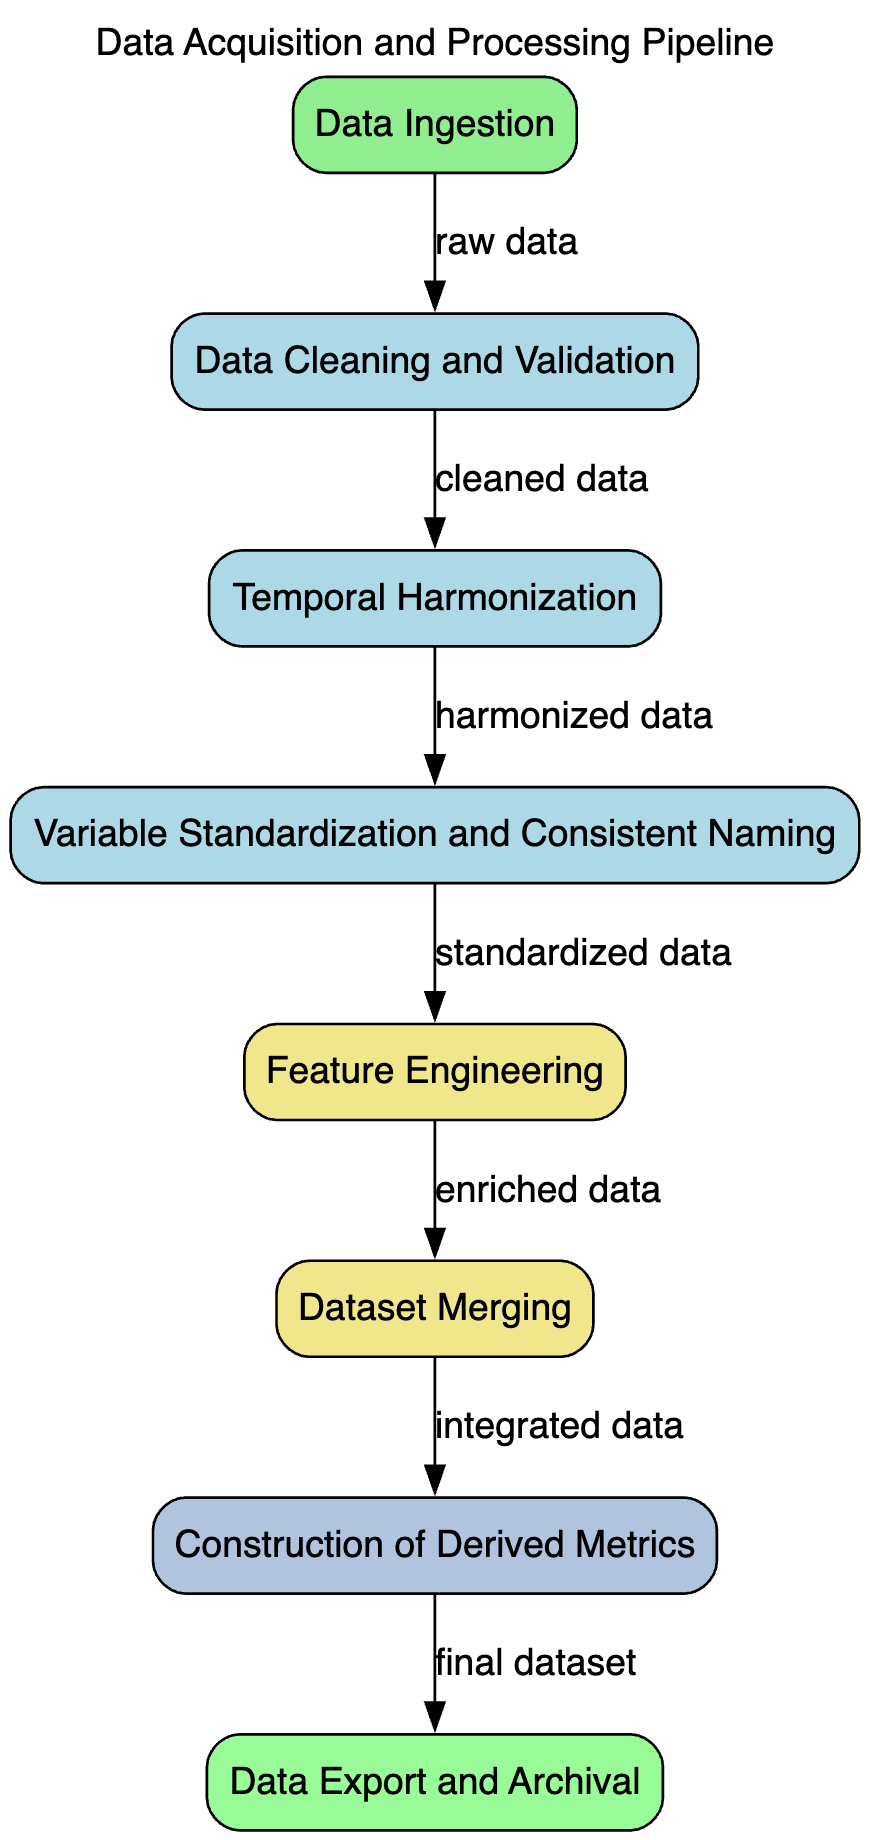
\includegraphics[width=0.8\textwidth]{images/dataacq.png}
\caption{Data acquisition and processing pipeline illustrating the systematic integration of diverse data sources through automated extraction, cleaning, harmonization, and feature engineering stages.}
\label{fig:data_pipeline}
\end{figure}

To reconcile discrepancies in reporting frequencies, temporal resolutions, and formats, multiple harmonization techniques were employed:

\begin{itemize}
  \item \textit{Temporal Alignment}: Monthly and quarterly series were aggregated to yearly values appropriate for the modeling time horizon. Arithmetic means were used for flow variables to preserve cyclical trends, while end-of-year snapshots were employed for stock variables such as interest rates to maintain economic state fidelity.
  
  \item \textit{Consistent Nomenclature}: Standardized variable naming conventions, such as \texttt{source\_variable\_annual}, were instituted for streamlined dataset merging and to avoid ambiguity.

  \item \textit{Missing Data Handling}: Observations exhibiting excessive missingness (>15\%) were excluded to prevent bias. Short gaps (less than three consecutive years) were imputed with seasonally informed linear interpolation, maintaining temporal continuity.

  \item \textit{Anomaly Detection}: Median absolute deviation (MAD) screening was applied to identify and remove outliers potentially arising from reporting errors or exceptional economic shocks.

  \item \textit{Vintage Control}: Macro series revisions were tracked through vintages to enable robustness analyses contrasting initial and finalized data releases, a critical consideration given known economic data revisions \citep{garcia2020}.
\end{itemize}

\subsection{Feature Engineering}\label{subsec:feature_engineering}

Enhancing the dataset's predictive and causal inference potential necessitated extensive feature engineering:

\begin{itemize}
  \item Introduction of lagged variables covering up to twelve prior years to capture long-range autocorrelations and regime dependencies, vital for effective sequence modeling with LSTM networks \citep{sekhansen2023}.

  \item Computation of growth rates, year-over-year percent changes, and relative deviations from historical means to expose transient macroeconomic shocks and cyclical fluctuations.

  \item Inclusion of rolling-window volatility measures and smoothed trend components (e.g., Hodrick-Prescott filter residuals) to differentiate underlying structural trends from noise.

  \item Creation of nonlinear interaction terms, such as unemployment times inflation, to capture synergistic policy responses and labor market dynamics.

  \item Encoding of lead and lag policy event windows, allowing localized causal effect estimation surrounding VAT adjustment periods.
\end{itemize}

\subsection{Microeconomic Firm-Level Data}\label{subsec:firm_data}

Firm-level data derived from the BDS panel were key to modeling heterogeneous treatment effects:

\begin{itemize}
  \item Extraction of annual counts of active firms and firm deaths, segmented by three-digit NAICS sectors.

  \item Calculation of survival rates as one minus the ratio of firm deaths over total firms within sector-year cells, effectively quantifying firm continuity amidst fiscal and macroeconomic policy shifts.

  \item Stringent cleaning protocols including removal of missing records, winsorization at the 1st and 99th percentiles to mitigate leverage by extremes, and temporal focus on 2000--2022 aligning with core policy evaluation periods.

  \item Utilization of early historical data for contextual visualization and exploratory validation.
\end{itemize}

\subsection{Quality Assurance and Validation}\label{subsec:data_quality}

Robustness of empirical findings is supported by rigorous data quality checks:

\begin{itemize}
  \item Automated schema validations ensured type correctness, unit consistency, and standardized naming.

  \item Domain-informed range checks eliminated structurally implausible values inconsistent with economic realities.

  \item Structural break detection applied Bai--Perron tests to identify temporal regime shifts and validate consistency with documented recessions or policy events.

  \item Revision tracking compared real-time and revised data impact on model estimates, quantifying sensitivity to data vintage.

  \item Manual anomaly quarantining involved expert reviews of flagged outliers prior to reinstatement for full analysis.
\end{itemize}

\subsection{Analytical Sample Composition}\label{subsec:analytical_sample}

The resultant analytical panel is a rigorously curated, multi-resolution macro--micro dataset suitable for integrated hybrid modeling. It encompasses:

\begin{itemize}
  \item Thirty-three annual periods spanning 1990 through 2022, ensuring comprehensive overlap of macro and micro data.

  \item Approximately 87 macroeconomic variables including both raw series and engineered transformations.

  \item Twelve detailed firm-level metrics including survival rates and firm dynamics proxies.

  \item Fifteen demographic covariates facilitating subgroup treatment effect heterogeneity and distributional impact assessments.
\end{itemize}

\subsection{Summary and Outlook}

This carefully constructed, multi-source dataset forms the backbone of the hybrid econometric-machine learning methodology developed in this thesis. By integrating reliable macroeconomic indicators, firm-level structural data, and demographic information alongside precise VAT policy markers, the empirical framework delivers robust forecasting, causal effect estimation, and nuanced heterogeneity detection. The succeeding methodological and empirical chapters build upon this foundation to advance VAT policy impact analysis.

\begin{figure}[htbp]
\centering
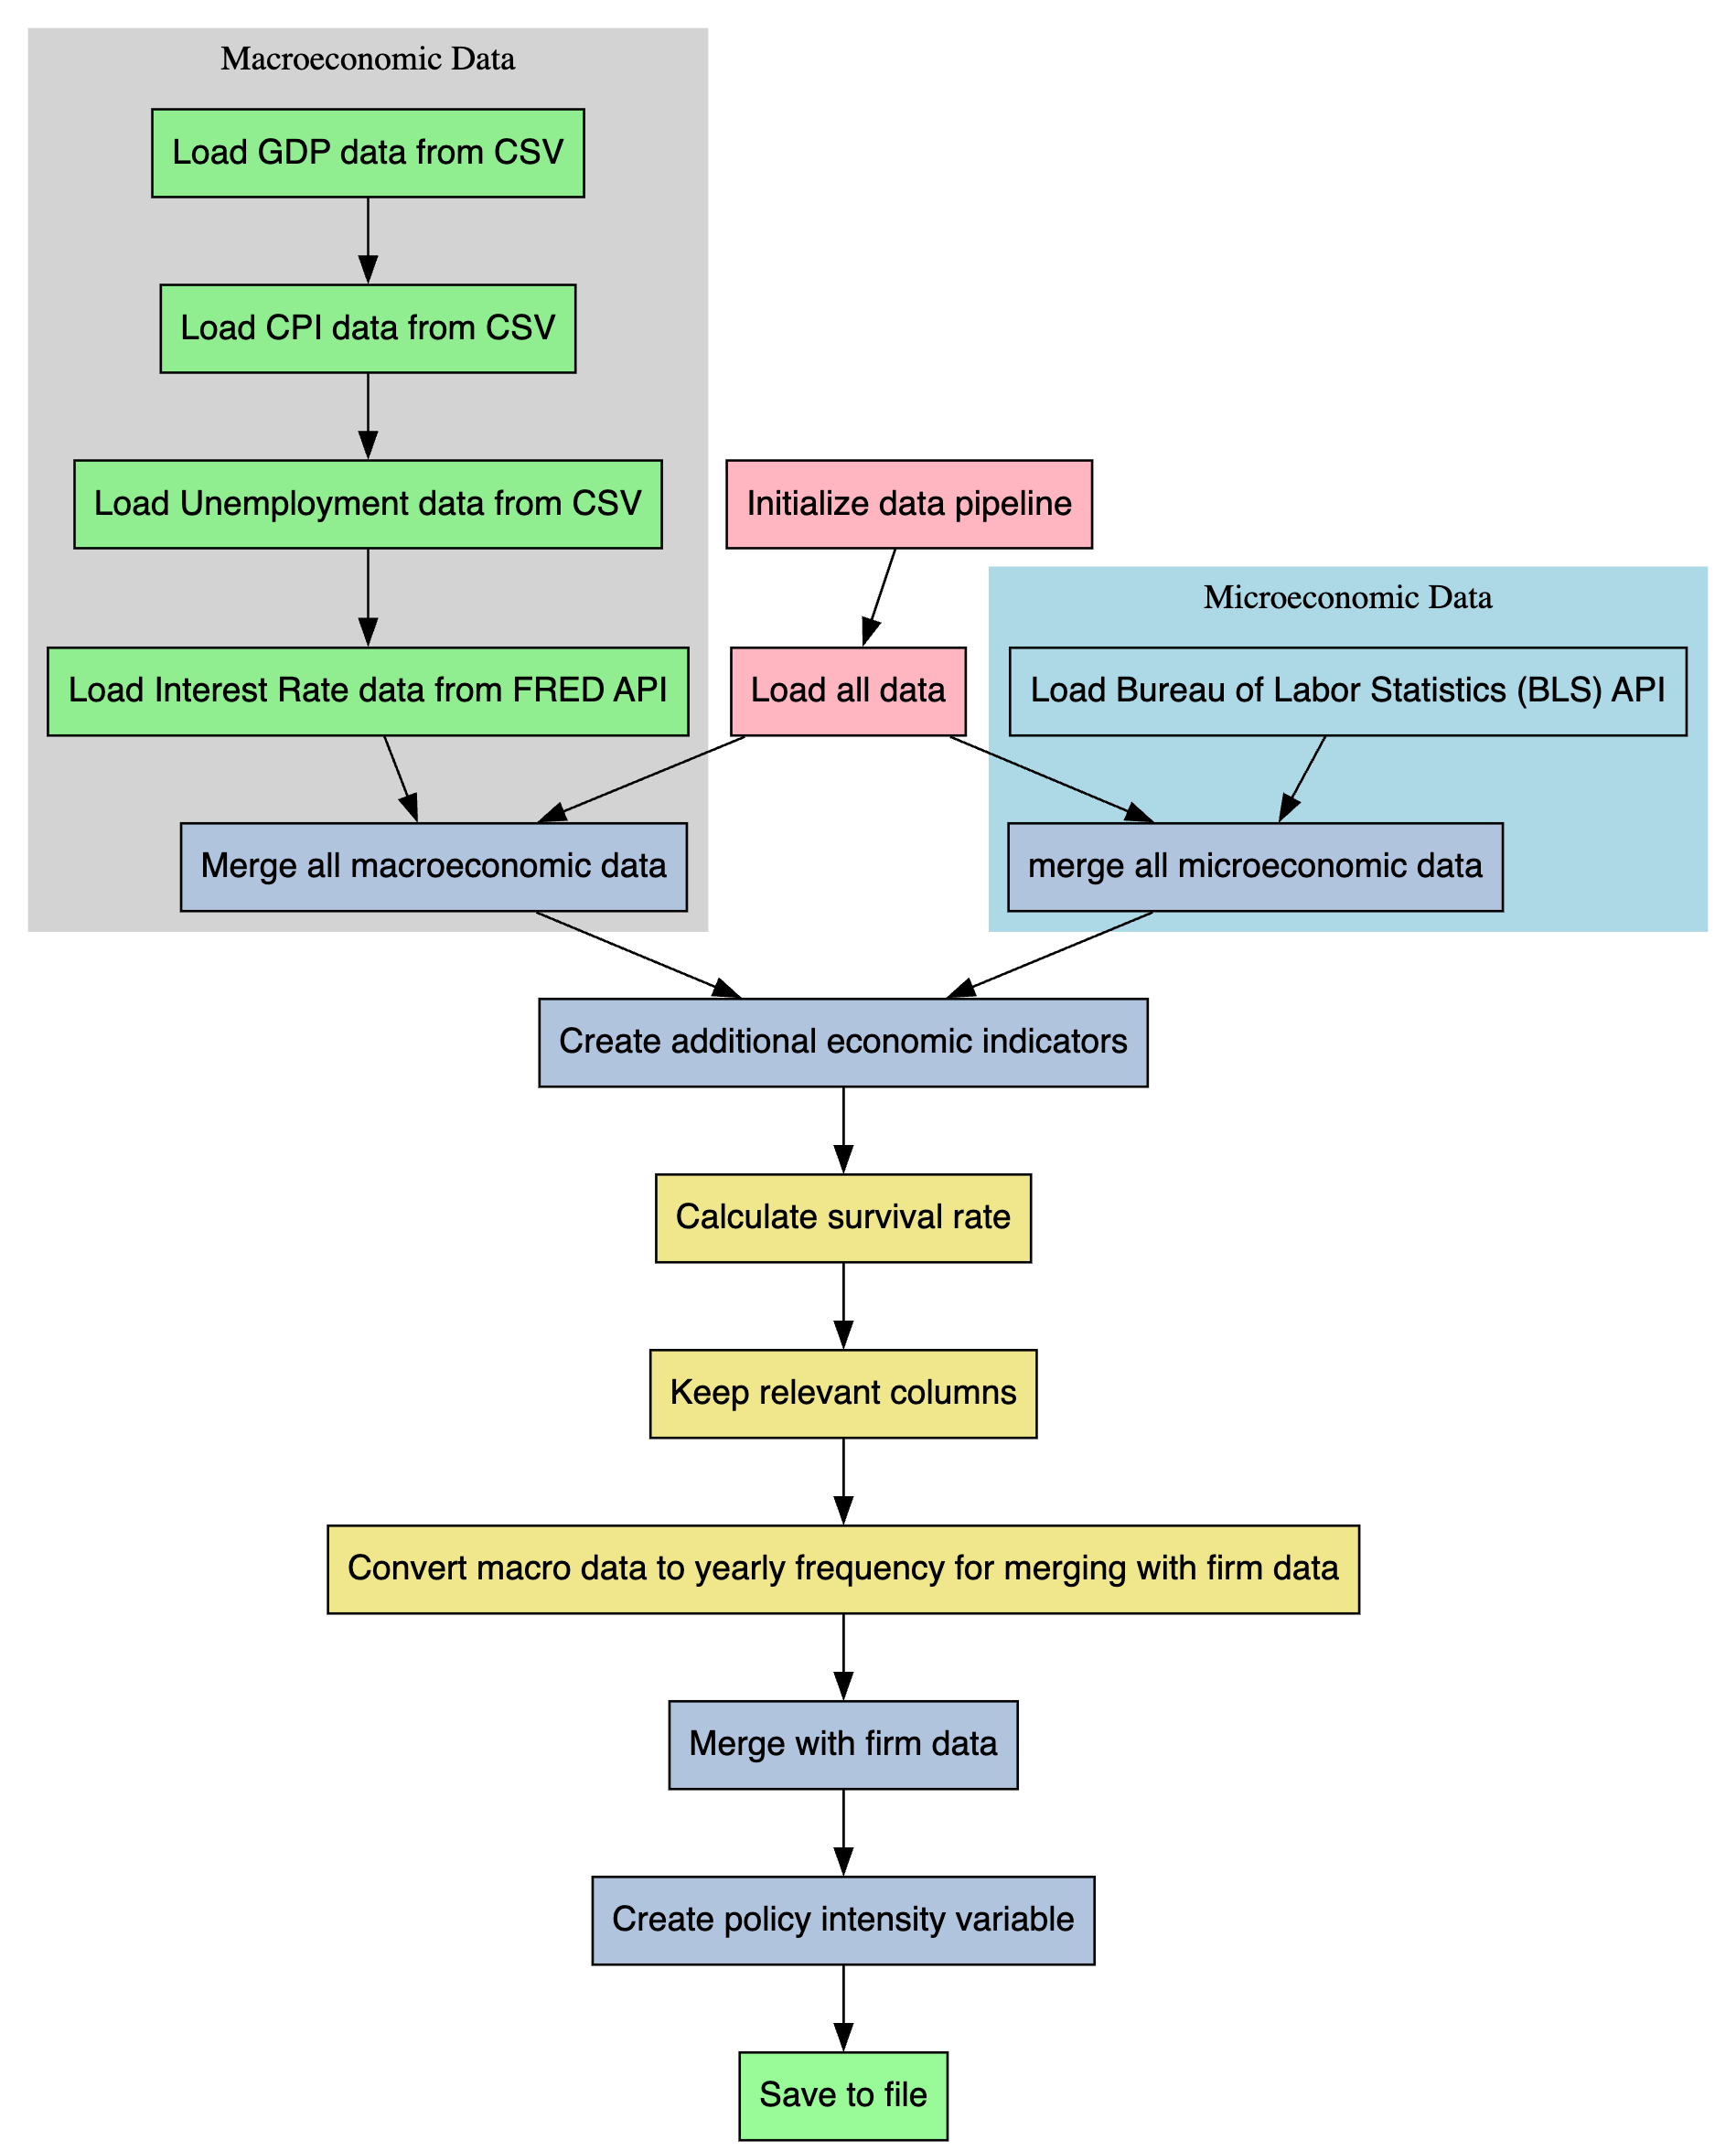
\includegraphics[width=0.8\textwidth]{images/wholedata.png}
\caption{Complete dataset overview showing the integration of macroeconomic indicators, firm-level data, and demographic variables across the analytical sample period.}
\label{fig:wholedata}
\end{figure}

